\section{Latency Development on Individual Months}
\label{sec:latency-individual-months}

We looked at the latencies within single months.

\subsection{Latencies on Different Weekdays}
\label{sec:latency-weekdays}

It is in question whether latencies vary at different days of the week. For
example, the latency might be different comparing Mondays and Sundays. In the
case of Starlink, we were not able to find such a pattern.
Figure~\ref{fig:latencies-per-weekday} illustrates the latencies that occurr in
each weekday.

\begin{figure}
	\centering
	\begin{subfigure}[b]{0.32\linewidth}
		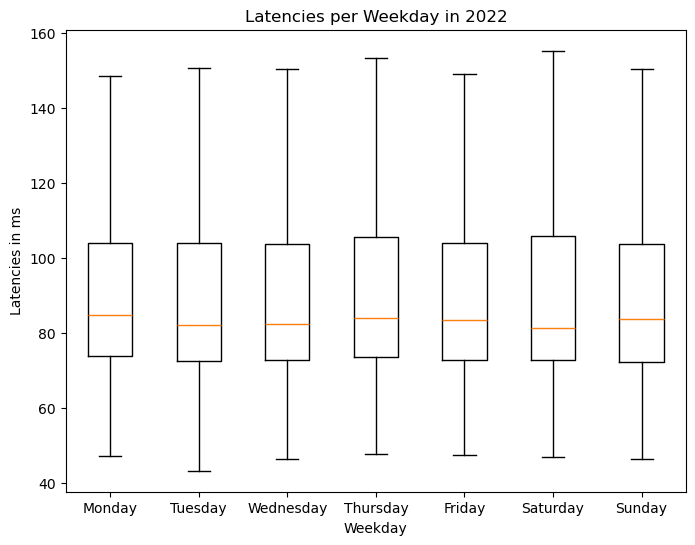
\includegraphics[width=\linewidth]{chapters/4-results/latency/img/latency_2022_weekdays.png}
	\end{subfigure}
	\begin{subfigure}[b]{0.32\linewidth}
		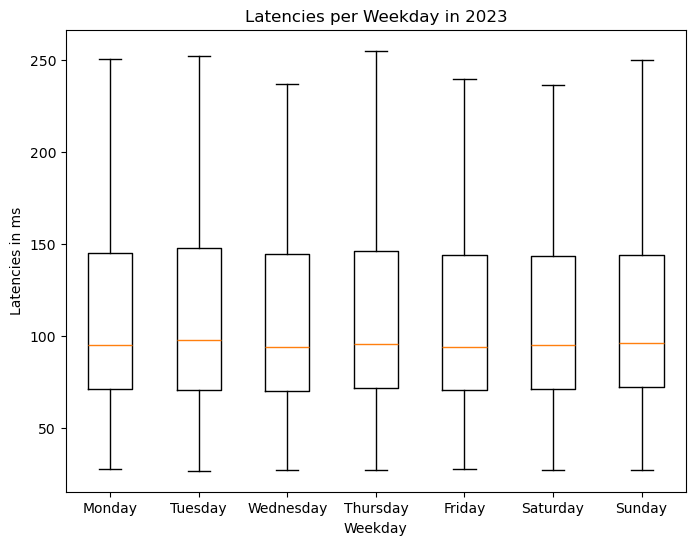
\includegraphics[width=\linewidth]{chapters/4-results/latency/img/latency_2023_weekdays.png}
	\end{subfigure}
	\begin{subfigure}[b]{0.32\linewidth}
		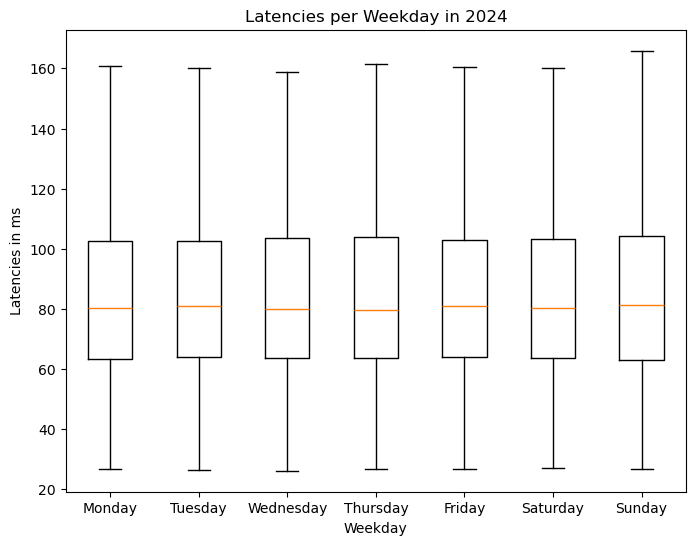
\includegraphics[width=\linewidth]{chapters/4-results/latency/img/latency_2024_weekdays.png}
	\end{subfigure}
	\caption{Latencies from 2022 to 2024 per Weekday.}
	\label{fig:latencies-per-weekday}
\end{figure}

One can see that there is no clear pattern that differentiates the individual
weekdays from the others. This does not change over the course of the years.

To look in more detail on the data, we looked at the data in specific
statistical aggregates (number of measurements, median, average, maximum, and
minimum latency). The results are shown in Table~\ref{fig:weekday-statistics}.

\begin{table}
	\caption{Weekday Statistics in Germany}
	\label{fig:weekday-statistics}
	\begin{tabular}{llllllll}
		\toprule
		               & Mon. & Tue. & Wed. & Thu. & Fri. & Sat. & Sun. \\
		\midrule
		\textbf{2022}  &      &      &      &      &      &      &      \\
		\#Measurements & 899  & 895  & 904  & 903  & 906  & 918  & 893  \\
		Median         & 84   & 82   & 82   & 84   & 83   & 81   & 83   \\
		Average        & 100  & 100  & 106  & 97   & 99   & 99   & 93   \\
		Maximum        & 1211 & 3090 & 3056 & 703  & 1229 & 1106 & 672  \\
		Minimum        & 47   & 43   & 46   & 47   & 47   & 47   & 46   \\
		\midrule
		\textbf{2023}  &      &      &      &      &      &      &      \\
		\#Measurements & 1448 & 1447 & 1443 & 1429 & 1430 & 1436 & 1462 \\
		Median         & 95   & 98   & 94   & 95   & 94   & 95   & 96   \\
		Average        & 111  & 111  & 108  & 109  & 107  & 108  & 108  \\
		Maximum        & 1245 & 1227 & 1233 & 707  & 1088 & 1220 & 1052 \\
		Minimum        & 28   & 26   & 27   & 27   & 27   & 27   & 27   \\
		\midrule
		\textbf{2024}  &      &      &      &      &      &      &      \\
		\#Measurements & 914  & 930  & 904  & 913  & 914  & 912  & 918  \\
		Median         & 80   & 81   & 80   & 79   & 81   & 80   & 81   \\
		Average        & 97   & 93   & 104  & 105  & 95   & 95   & 95   \\
		Maximum        & 3147 & 1592 & 4374 & 3624 & 4368 & 1230 & 1320 \\
		Minimum        & 26   & 26   & 26   & 26   & 26   & 27   & 26   \\
		\bottomrule
	\end{tabular}
\end{table}

They show that the latency does not vary on the individual days. Therefore, you
will not have a worse latency on working days (Mon. -- Fri.) compared to the
weekend (Sat. and Sun.).

However, the table also allows for an interesting comparison between the years
2022, 2023, and 2024. In 2022, the median latency was between 81 and 84 ms. The
average latency was about 20 ms higher. Peak latencies achieved up to 43 ms. In
2023, the median latencies were significantly higher at 94 to 98 ms. The
average latency was in the worst case 14 ms higher, which indicates a more
stable connection, even if the performance was worse compared to 2022. However,
2023 achieved much better peak performance at 26 ms. In 2024, Starlink achieved
similar median and average latencies compared to 2022, but also achieving the
peak performances from 2023.

\begin{takeaway}{Peak and Average Latency since 2022.}
	Starlink has managed to improve their peak latency compared to 2022 by
	nearly 20 ms while maintaining their median and average latencies.
\end{takeaway}

\begin{figure}
	\centering
	\begin{subfigure}[t]{0.47\linewidth}
		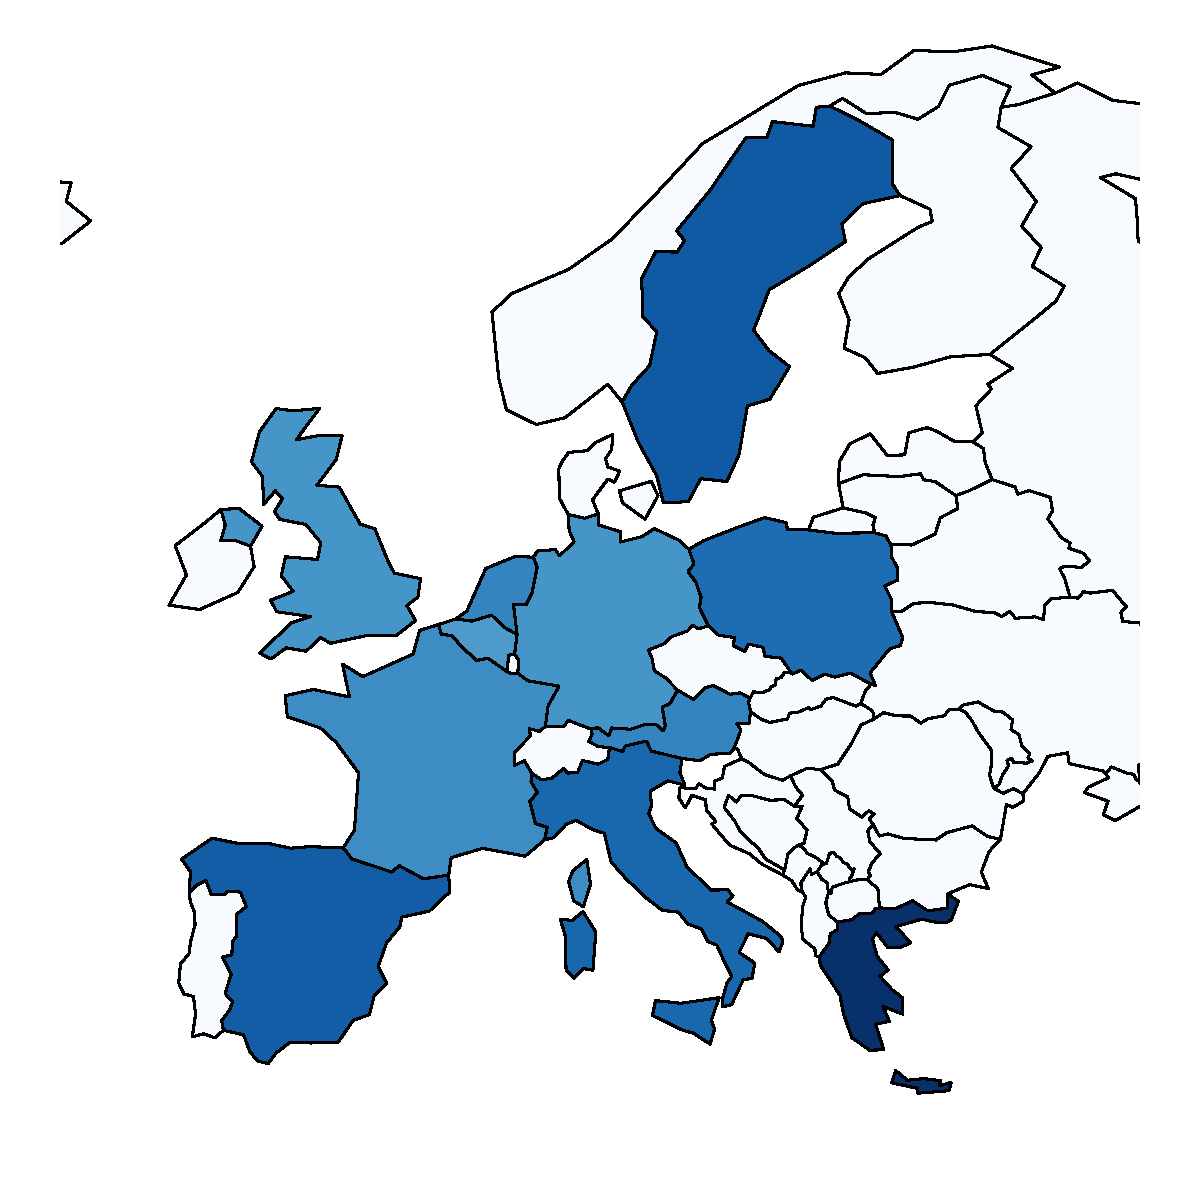
\includegraphics[width=\linewidth]{chapters/4-results/latency/img/heatmap-median-latencies-2024.pdf}
		\caption{Median}
	\end{subfigure}
	\begin{subfigure}[t]{0.47\linewidth}
		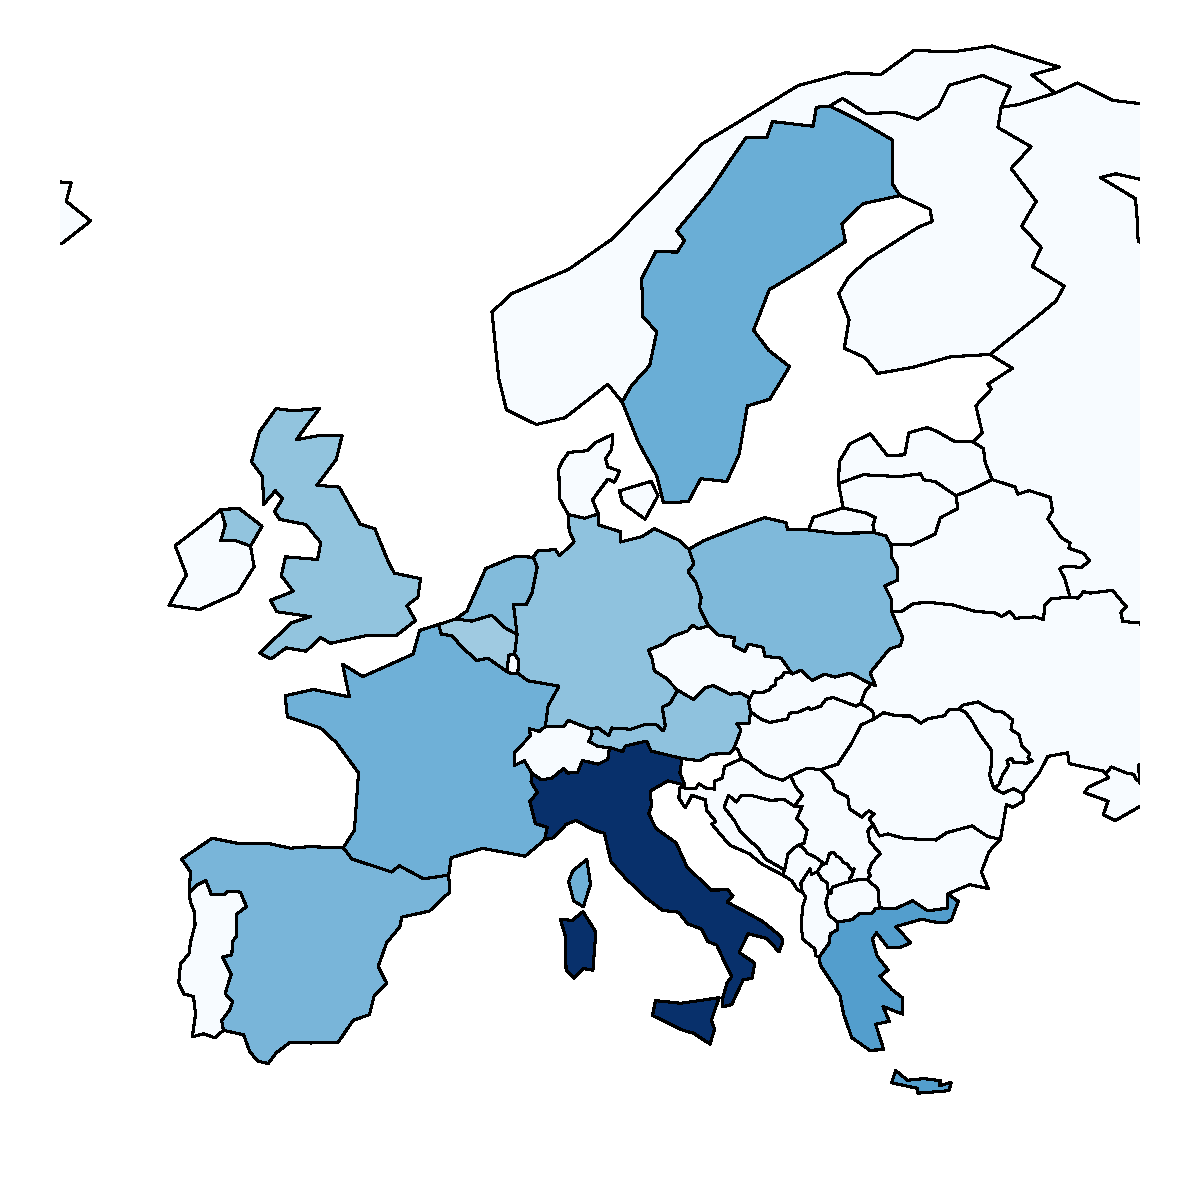
\includegraphics[width=\linewidth]{chapters/4-results/latency/img/heatmap-average-latencies-2024.pdf}
		\caption{Average}
	\end{subfigure}
	\caption{Heatmap of Median and Average Latencies in 2024 in Europe
		(darker color means a higher latency).}
	\label{fig:heatmap-latencies-europe}
\end{figure}

Figure~\ref{fig:heatmap-latencies-europe} shows the median and average
latencies in European countries. It shows that the north-west of Europe
experiences the best latencies, likely due to the presence of various \ac{GS}s.
The southern and eastern European countries experience worse latencies.
Especially Greece has a high median latency. A cause could be the absence of
\ac{GS}s in the east European region. Italy on the other hand side experiences
a high average latency, even with \ac{GS}s being present in the country.

